\documentclass[a4paper,12pt]{article}
\usepackage[utf8]{inputenc}
\usepackage[czech]{babel}
\usepackage[T1]{fontenc}
\usepackage[left=3.5cm,right=2cm,top=3cm,bottom=3cm]{geometry}
\usepackage{amsmath,amsfonts,amssymb}
\usepackage{enumerate}
\usepackage{gensymb,marvosym}
\usepackage{times}
\usepackage{tabularx}
%\usepackage{graphicx}
\usepackage{xparse}
\usepackage{pdfpages}

% Nastavení pevných mezer za jedno a dvou znaková slova
\ExplSyntaxOn
  \tl_new:N \l_wave_tmpa_tl
  \cs_new:Npn \wave_putter:n #1 {
      \tl_set:Nn \l_wave_tmpa_tl { #1 }
      \regex_replace_all:nnN {([\ \t\n\-\x{28}]{1})(.{1,3})([\ \t\n]{1})} {\1\2\-} \l_wave_tmpa_tl
      \regex_replace_all:nnN {([\ \t\n\-\x{28}]{1})(.{1,3})([\ \t\n]{1})} {\1\2\-} \l_wave_tmpa_tl
      \tl_use:N \l_wave_tmpa_tl
  }
  \cs_generate_variant:Nn \wave_putter:n { e }

  \NewDocumentCommand \wavePutter { m } {
    \input{ content/#1 }
    \wave_putter:e { #1 }
    %\wave_putter:e { Some text
 }
    %\wave_putter:e { \section{Second section} }
  }
\ExplSyntaxOff

\usepackage[
  backend=biber,        % defaultní možnost, nastaví unicode a několik dalších vlastností
  style=iso-numeric,    % iso-numeric pro číselné uspořádnání nebo iso-authoryear pro uspořádání pomocí autorů
]{biblatex}

\addbibresource{literatura.bib}

% Více řádků v jednom pro tabulku
\usepackage{multirow}

% Pro tečkovanou čáru pro podpis
\usepackage{arydshln}

\usepackage[none]{hyphenat} \sloppy
\clubpenalty 10000
\widowpenalty 10000

% Nastavení řádkování
\usepackage{setspace} \onehalfspacing

% === Nastavení hlavních proměnných ===
\newcommand{\autor}{Jiří Alexandrovič}
\newcommand{\skola}{Česká zemědělská univerzita v Praze}
\newcommand{\fakulta}{Technická fakulta}
\newcommand{\nazev}{Technické prostředky informačních systémů}
\newcommand{\vedouciPrace}{Ing. Jan Lešetický, Ph.D.}
\newcommand{\typPrace}{bakalářská práce}


% Nastavení prolinkování odkazů v dokumentu
\usepackage[pdftex,
  pdfauthor={Jiri Alexandrovic},
  pdftitle={Technicke prostredky informacnich systemu},
  pdfsubject={},
  pdfkeywords={},
  pdfproducer={Ceska zemedelska univerzita},
  pdfcreator={pdflatex}]{hyperref}

\hypersetup{
    colorlinks = false,
    hidelinks
}

\usepackage{fancyhdr}
%\usepackage{graphicx}

% Nastavení cesty k obrázkům
\graphicspath{{pics/}}

% Funkce pro vkládání grafů
\usepackage{float}
\newfloat{graf}{hbtp}{ext}
\floatname{graf}{Graf}

% Pojmenovaní obrázku
\usepackage{caption}
\captionsetup[figure]{name=Obr.}

% === Začátek dokumentu ===
\begin{document}
\pagestyle{empty}

%\begin{titlepage}
	\centering

  \vfill

	{\LARGE \skola \par}
	{\Large \fakulta \par}

	\vfill

	{\huge\bfseries \nazev \par}
	{\Large \typPrace \par}

  \vfill

  {\Large Vedoucí práce: \vedouciPrace \par}
	{\Large Autor práce: \autor \par}

	\vspace{1.5cm}

	{\scshape\large \misto ~ \the\year \par}

  \vfill
\end{titlepage}


% Vložení strány se zadáním
%\newgeometry{left=0cm,right=0cm,top=0cm,bottom=0cm}
%
\includegraphics{../zadani.pdf}
%\restoregeometry
%\clearpage


%\vspace*{\fill}
\section*{Čestné prohlášení}
Prohlašuji, že jsem diplomovou/bakalářskou práci na téma: \inserttitle \ vypracoval/a samostatně a použil/a jen pramenů, které cituji a uvádím v seznamu použitých zdrojů.

Jsem si vědom/a, že odevzdáním bakalářské práce souhlasím s jejím zveřejněním dle zákona č. 111/1998 Sb., o vysokých školách a o změně a doplnění dalších zákonů, ve znění pozdějších předpisů, a to i bez ohledu na výsledek její obhajoby.

Jsem si vědom/a, že moje bakalářská práce bude uložena v elektronické podobě v univerzitní databázi a bude veřejně přístupná k nahlédnutí.

Jsem si vědom/a že, na moji bakalářskou práci se plně vztahuje zákon č. 121/2000 Sb., o právu autorském, o právech souvisejících s právem autorským a o změně některých zákonů, ve znění pozdějších předpisů, především ustanovení § 35 odst. 3 tohoto zákona, tj. o užití tohoto díla.

\qquad

\setlength{\dashlinedash}{1pt}
\setlength{\dashlinegap}{1pt}
\setlength{\arrayrulewidth}{1pt}

\noindent
\begin{tabularx}{\textwidth}{X r}
V Praze dne \today &
\begin{tabular}[b]{@{} p{6cm} @{}}
\\
\hdashline
\centering
podpis
\end{tabular}
\\
\end{tabularx}


%% === Poděkování ===
% Není možné děkovat komisi nebo oponentovi práce.
\vspace*{\fill}
\section*{Poděkování}
Rád bych poděkoval svému vedoucímu práce panu "vedoucí Práce", za výběr tématu a možnost pracovat pod jeho vedením. Díky tomuto tématu jsem získal mnoho znalostí, které mohu uplatnit v praxi. Dále bych chtěl poděkovat ...


% === Nastavení obsahů pro dokumenty ===
% tabulka s obsahem
%\tableofcontents

% seznam zkratek
% pouze u většího množství zkratek
%\include{seznamZkratek}

% seznam tabulek
% pouze pokud jsou použity více jak tři tabulky
%\newpage
%\listoftables
%\thispagestyle{empty}

% seznam obrázků
% pouze pokud jsou použity více jak tři obrázky
%\newpage
%\listoffigures
%\thispagestyle{empty}

\setcounter{page}{1} %cislo strany
\thispagestyle{empty}
%\pagestyle{empty}

\newpage

\pagestyle{fancy} %vlastni zahlavi/zapati
\renewcommand{\headrulewidth}{0.5pt} %bez linky v zahlavi
\renewcommand{\footrulewidth}{0pt} %linka v zapati
\lhead{\leftmark}       \chead{} \rhead{} %pole zahlavi (prazdna)
\lfoot{} \cfoot{} \rfoot{\thepage} %pole zapati


\newcommand{\myNewCommandIsIMBA}[1]{\input{./content/{#1}}}

%\wavePutter{Test test A a a a t test test. No a taky už ještě ž týden.}

%\wavePutter{\skola}

\wavePutter{01obsah}

obsah a nějaký text~\cite{ref:proc:powersaving2}

%\section{Základní desky}
Základní deska v angličtině motherboard nebo také mainboard je jedena z nejdůležitějších
součástí počítačové sestavy. Základní deska je deskou s tištěnými spoji v literatuře PCB\footnote{Z anglického prited circuit board}.

Jedná se o součást, která vytváří mechanickou podporu a hlavně elektrické propojení jednotlivých elektronických součástí
nebo elektrických komponent pomocí vodivých spojů. Je to také největší tištěný spoj v počítačové sestavě.

\subsection{Konstrukce a vývoj}
Základna základní desky je tvořena velice pevným a nevodivým materiálem. Obvykle se jedná
o téměř jakýkoliv druh tuhého plastu. Na tuto desku jsou následně natištěny tenké vrstvy
měděné nebo hliníkové fólie.\cite{ref:mb:study} Tyto vrstvy jsou označovány anglickým názvem traces,
což by se dalo přeložit jako cesty nebo trasy. Jsou takto pojmenovány kvůli tomu, že plní
funkci spojů jednotlivých komponent.

Základní desky sice nemají stejnou konstrukci je však několik charakteristik, které je spojují.
Jedny z hlavních jsou integrované obvody nordbridge nebo-li severní můstek a southbridge nebo-li jižní můstek.
Slouží ke komunikaci CPU s pamětí a I/O porty\footnote{Vstupně výstupní porty. Z anglického Input/Output.}.

\subsubsection{Nordbridge}
Nordbridge je připojen přímo k CPU pomocí front side bus (FSB obrázek
č.~\ref{fig:chipset}), což je obousměrná datová sběrnice.
Obrázek č.~\ref{fig:chipset} starší schéma, na kterém nordbridge obsahoval
například paměťovou sběrnici, ta sloužila jako řadič pro
pamět RDRAM. Dále nordbridge obsahuje sběrnici pro grafickou kartu. Na obrázku
je popsána AGP nebo PCI-E, protože se jedná o dvě různá rozhraní.

AGP (z anglického Accelerated Graphics Port) je navrženo pro aplikace
používající 3D grafiku. AGP je kanál využívající point-to-point\footnote{Dvoubodový
spoj zajišťující komunikaci mezi právě dvěma uzly.}, díky kterému
je zajištěn přímý přístup k hlavní paměti. Poskytuje šířku pásma
od $266 Mbps$ do $1,07 Gbps$~\cite{ref:mb:onlinecomputertips}.

PCI-Express rozšiřuje a zvětšuje přenosovou rychlost standardního
rozhraní PCI. Je to obousměrné sériové připojení (point-to-bus),
které zabraňuje
problémům s výkonem. Ty mohou nastat při sdílení šířky
pásma na sběrnici. Na rozdíl od AGP je možné toto rozhraní
použít i s jinými zařízeními jako jsou
síťové karty k dosažení větší propustnosti než u standardního
PCI~\cite{ref:mb:onlinecomputertips}.

Kvůli trendu integrace většího množství funkcí do méně součástí byl například
řadič pro komunikaci mezi CPU a RAM přesunut do procesoru.
Tato změna má výhodu v tom, že snižuje celkové
náklady na výrobu základních desek a snižuje latenci mezi
CPU a pamětí, díky čemuž se zvýší výkon \cite{ref:mb:srgtech}.

\begin{figure}[htbp]
  \centering
  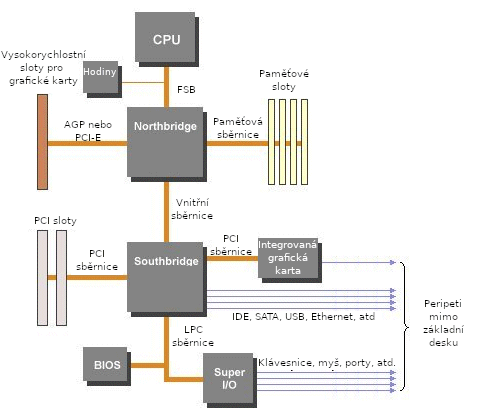
\includegraphics[width=12cm]{chipset.png}
  \caption{Schéma chipsetu na základní desce.~\cite{ref:mb:technologyuk}}
  \label{fig:chipset}
\end{figure}

\subsubsection{Southbridge}
Southbridge bývá menší než nordbridge a zajišťuje pomalejší funkce základní desky.
Tomuto také odpovídá jeho umístění, které je dál od CPU. Southbridge může
obvykle obsluhovat i více jak jeden nordbridge. Neexistuje však standard pro
vzájemnou komunikaci, kvůli tomu musí oba čipy pro vzájemnou kompatibilitu navrženy.

Dříve se pro komunikaci mezi southbridge a nordbridge používala sběrnice PCI,
toto spojení však nízkou propustnost. Většina současných chipestů tedy používá
pro komunikaci proprietální rozhraní~\cite{ref:mb:edusoft}.

Na obrázku č. \ref{fig:chipset} je vidět, že southbridge má PCI sloty. PCI
(z anglického Peripheral Component Interconnect) je nejstarším řadičem
pro grafické karty. Dnes se spíše pro zvukové nebo síťové karty, protože
pro grafické karty nemusí mít dostatečnou propustnost, lze ho však používat s grafickými kartami, které mají na své desce hodně paměti. PCI umožňuje komunikaci mezi
různými zařízeními na sběrnici. Poskytuje šířku pásma až $133 Mbps$ a 64 bitová
verze podporuje až $512 Mbps$~\cite{ref:mb:edusoft}.


\subsection{BIOS}
Zkratka pochází z anglického Basic Input/Output System. Je to čip typu ROM,
který se nachází na základní desce a umožňuje zavedení systému počítače.
Bios obsahuje instrukce pro zavedení základního hardwaru počítače. BIOS
obsahuje také POST (Power-On Self-Test), který slouží k ověření požadavků
pro správné nabootování (naběhnutí) systému. Pokud tento test neprojde, BIOS
pomocí pípání oznámí, jaký problém nastal~\cite{ref:mb:techtarget}.

Hlavními úkoly, které BIOS zastává jsou výše zmíněný POST, dále Bootstrap Loader,
BIOS drivers, BIOS setup. Bootstrap Loader se snaží najít
operační systém a pokud se mu to podaří, předá mu řízení. BIOS drivers obsahuje
nízkoúrovňové ovladače pro základní komunikaci s hardwarem
a BIOS setup, někdy se mu také říká CMOS setup, konfiguruje program, který
umožní nastavení hardwaru počítače~\cite{ref:mb:computerhope}.

Na obrázku č. \ref{fig:bios} je vidět čip AMBIOS z roku 1995 od firmy AMI\footnote{Společnost
American Megatrends, Inc.}, která se specializuje na PC hardware a firmware.

\begin{figure}[htbp]
  \centering
  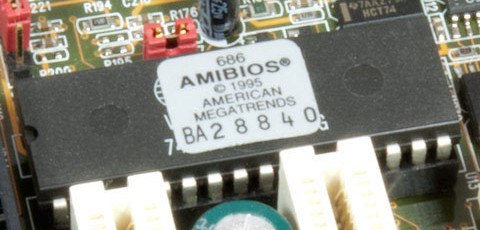
\includegraphics[width=12cm]{bios.jpg}
  \caption{AMBIOS typ BIOSu od společnosti AMI.~\cite{ref:mb:computerhope}}
  \label{fig:bios}
\end{figure}

\subsubsection{Upgradování a updatování}
Upgradování jakožto přidání další paměti pro BIOS je možné pouze tak, že se fyzicky odebere čip obsahující BIOS ze základní desky a posléze přidání
novějšího čipu.

BIOS je však možné updatovat, pokud se jedná o flash BIOS. Flash BIOS je možné
spustit pomocí speciálního disku nebo provést sadu instrukcí,
které BIOS updatují bez nutnosti fyzického zásahu do základní
desky~\cite{ref:mb:itstillworks}. Pomocí takovéhoto updatu je možné opravit
problémy, či přidat nové funkce pro základní desku.

\subsection{Periferie a rozhraní základních desek}
Na základní desce můžeme najít další rozšiřující sloty v angličtině expansion slot,
bus slot nebo expansion port. Jedná se o konektory na základní desce nebo
na rozšiřující desce\footnote{Deska tištěných obvodů umožňující přidání
karet. V angličtině Riser card.}, které umožňují přidání rozšiřujících karet
do základní desky~\cite{ref:mb:computerhope2}.

V seznamu jsou uvedeny běžné rozšiřující karty, některé jsou však dnes již
zastaralé. V dnešní době se jsou běžné pouze AGP, PCI a PCI Express, které jsou
popsané výše.

\begin{itemize}
  \item AGP - grafické karty
  \item PCI - síťové, zvukové, grafické karty, SCSI\footnote{Z anglického
  Small Computer System Interface. Jde o rozhraní pro připojení pevných disků,
  skenerů, jednotky CD-ROM nebo DVD~\cite{ref:mb:webopedia2}.}
  \item PCI Express - síťové, zvukové, grafické karty, modemy
  \item AMR - modem, zvukové karty
  \item CNR - modem, síťové, zvukové karty
  \item EISA - SCSI, síťové, grafické karty
  \item ISA - síťové, zvukové, grafické karty
  \item VESA - grafické karty
\end{itemize}

Zkratka AMR je z anglického Audio/Modem Riser, jde o rozšiřující slot navržený
společností Intel. Zajišťuje analogovou funkcionalitu. Jeho nevýhodami je,
zabírá jeden slot pro PCI, nepodporuje plug and play\footnote{Automatické
používání po připojení bez nutnosti instalování ovladačů} a neumožňuje
hardwarovou akceleraci~\cite{ref:mb:pinouts}.

CNR je zkratka pro Comunication and Network Riser. CNR byl potenciální
úsporou nákladů tím, že by bylo možné odstranit analogové I/O komponenty
ze základních desek. To zlehčilo certifikaci u FCC. Celým jménem Federal
Communications Commission, je obdobou ČTK pro USA. To mělo za následek zmenšení
času potřebného k výrobě nových základních desek~\cite{ref:mb:pinouts2}.

Port EISA má název podle The Extended Industry Standard Architecture. Je
standardem pro sběrnice kompatibilní s PC IBM. EISA má 32 bitů a umožňuje sdílení
sběrnic mezi více CPU. Je také vylepšena pro to, aby mohla přistupovat k 4 GB paměti.
Mezi výrobci byla EISA velmi oblíbená a dokonce i firma IBM vyrobila některé
stroje, které ji podporovaly. Díky její vyšší nákladnosti se však příliš nerozšířila
na stolní počítače, ale měla spíš místo na trhu serverů~\cite{ref:mb:geekdot}.

ISA je název pro Industry Standard Architecture. Je to 16 bitová interní sběrnice
používající se u IBM PC/AT\footnote{Označení pro třetí generaci IBM PC}. IBM sběrnici také
označována jako I/O Channel. ISA byla základem pro pozdější vytvoření 32 bitové
sběrnice EISA~\cite{ref:mb:hardwarebook}

VESA, VESA Local Bus nebo také VL-Bus. Její vývoj zajišťovala VESA Committe\footnote{Zkratka
pro Video Electronics Standard Association.}. VL-Bus nabízel přímý přistup
do systémové paměti a to rychlostí podobnou procesoru. Data byla přenášena 32 bity,
výhodou toho bylo, že bylo možné zajistit vyšší tok dat mezi CPU a grafickou
kartou~\cite{ref:mb:karlstechnology}. Nevýhodou je však závislost na sběrnici
procesoru Intel 80486, s nástupem procesorů pentium došlo k rozdílům v konstrukci
sběrnice, které se nedaly snadno přizpůsobit. Navíc s rostoucí rychlostí systémů
486 se VL-Bus stával stále složitějším na ovládání a jeho design, který mu zajišťoval těsné spojení s místní sběrnicí se stával stále méně přizpůsobivým frekvenčním
změnám~\cite{ref:mb:atarimagazines}.

\subsection{Provedení pro stanice a servery}
Server sice lze sestavit i z běžných komponent, server má však jiná kritická místa
a je tedy nutné pro aplikace na kterých bude velké ztížení mít i specifický hardware.
Je však nutné pro i pro každý jednotlivý server zvolit správnou základní desku
podle potřeb daného serveru.

Server jako takový musí běžet nepřetržitě a bylo by velice problematické,
kdyby došlo k jeho pádu. S tím souvisí požadavky na snadnou modularitu a výměnu
komponent, které je v ideálním případě možné vyměňovat i za chodu
serveru~\cite{ref:mb:neweggbusiness}.

Navíc pokud server není určen pro opravdu velké firmy nebo instituce, je možné
slevit z nároků na jeho výkon. Tento parametr se však odvíjí hlavně od toho,
jak bude server využíván~\cite{ref:mb:neweggbusiness}.
Toto kritérium je však velice důležité pro to, kolik bude na serveru potřebné
operační paměti a procesorů, což má přímý dopad na základní desku, která musí
mít pro tyto požadavky vhodné periferie.

U serveru se tedy neuvádí propustnost
paměti a frekvence procesoru, ale počet transakcí, které server zvládne za sekundu
a hlavně počet I/O operací, které jsou nejspíše nejdůležitějším parametrem
serveru.

\subsection{Vývoj do budoucna}
Jak bylo popsáno výše, je trend přemisťování některých prvků, hlavně u CPU a GPU
do čipů, neboli takzvaný SOC\footnote{Z anglického System on a chip}. Dá se také
předpokládat, že paměťové porty se budou zrychlovat a bude se zvětšovat i
jejich hustota~\cite{ref:mb:embedded}.

Na druhou nic nenasvědčuje potřebě měnit
nějakým razantním způsobem kostru celé základní desky, tedy se dá předpokládat,
ta zůstane bez jiných než designových změn. Možná je však změna kostry základních
desek v zařízeních. Tam je však obtížné předpokládat jaký bude vývoj.

Také se pravděpodobně budou rozšiřovat využití různých speciálních zařízení, jako
jsou například chytré televize, které používají technologii DLNA pro připojování
k domácím mediálním serverům nebo osobním počítačům.

Na technologii DLNA, což je zkratkou pro Digital Living Network Aliance se podílí
velké množství předních výrobců spotřební elektroniky. Tato technologie se snaží hlavně o to, aby bylo možno vytvořit domácí bezdrátovou síť, ve které jsou schopné AV systémy
spolu s počítači a mobilními zařízeními sdílet multimediální obsah, bez toho
aby bylo nutné tyto zařízení konfigurovat~\cite{ref:mb:embedded}.

%\myNewCommandIsIMBA{01obsah}

%\section{Some section}

Here is some examples, how to use basics for document.

\begin{itemize}
  \item Citation~\cite{ref:proc:powersaving2}.
  \item Footnote text\footnote{Here is some description.}
  \item Reference to picture č.~\ref{fig:pic}, graph~\ref{grp:graph}, table~\ref{tbl:table}.
\end{itemize}

\insertpicture[fig:pic]{tux.png}{5cm}{We love linux.}

\insertgraph[grp:graph]{graph.png}{12cm}{We love \LaTeX.}

\begin{inserttable}[tbl:table]{|l|c|r|}{Some table example.}
  \hline
  Here       & is      & some     \\ \hline
  ultimately & amazing & example. \\ \hline
\end{inserttable}


\clearpage

% === Zdroje ===
\phantomsection % přidání odkazu do PDF záložek
\addcontentsline{toc}{section}{Seznam použitých zdrojů}
\renewcommand{\refname}{Seznam použitých zdrojů}

\printbibliography

\end{document}
